\documentclass[aspectratio=169, 11pt]{beamer}

% --- Tema minimalista ---
\usetheme{default}
\usecolortheme{default}
\usefonttheme[onlymath]{serif}
\setbeamertemplate{navigation symbols}{}
\setbeamertemplate{footline}[frame number]
\setbeamercolor{footline}{fg=gray}
\setbeamercolor{frametitle}{fg=black}
\setbeamerfont{frametitle}{size=\large}
\setlength{\leftmargini}{0pt}

\usepackage[utf8]{inputenc}
\usepackage[spanish]{babel}
\usepackage{graphicx}
\usepackage{amsmath,amssymb}
\usepackage{hyperref}
\usepackage{booktabs}
\usepackage{tabularx}
\usepackage{multirow}

\graphicspath{{figures/}}

\title{Simulación computacional de dinámica de fluidos\\para el análisis hemodinámico de la enfermedad coronaria}
\author{Juan José Zuluaga Patiño}
\institute{Universidad del Rosario}
\date{2026}

\begin{document}

% ---------------------------------------------------------------
\begin{frame}[plain]
  \centering
  \vspace{0.5cm}
  {\small\textcolor{gray}{Universidad del Rosario}}
  \vfill
  {\large\textbf{Simulación computacional de dinámica de fluidos\\para el análisis hemodinámico de la enfermedad coronaria}}
  \vfill
  {\small Juan José Zuluaga Patiño} \\
  {\small\textcolor{gray}{Director: José Alejandro Guerrero Vargas, PhD}}
  \vfill
  
\includegraphics[height=0.5cm]{urosario_logo.png}
\end{frame}

% ---------------------------------------------------------------
\begin{frame}{Problema clínico}
  % La enfermedad arterial coronaria (EAC) es una de las principales causas de muerte global. Se caracteriza por el estrechamiento (estenosis) de las arterias que irrigan el corazón. La aterosclerosis es la causa subyacente: acumulación de placa en las paredes arteriales.

  \centering
  \vfill
  {\Large\textbf{Enfermedad Arterial Coronaria (EAC)}}
  \vspace{0.5cm}

  \textcolor{gray}{$\uparrow$ Principal causa de muerte a nivel mundial}

  \vspace{1cm}
  \textcolor{gray}{\small Estrechamiento progresivo de arterias coronarias por aterosclerosis}
  \vfill
\end{frame}

% ---------------------------------------------------------------
\begin{frame}{Diagnóstico actual}
  % El diagnóstico tradicional se basa en imágenes anatómicas: angiografía invasiva (ICA) o por tomografía (CTCA). El problema: la severidad anatómica NO siempre se correlaciona con el impacto fisiológico (isquemia). Muchas lesiones "intermedias" son difíciles de evaluar.

  \centering
  \vfill
  {\large\textbf{Anatomía $\neq$ Fisiología}}
  \vspace{0.5cm}

  \textcolor{gray}{Angiografía: excelente detalle anatómico, \\ pero la severidad visual no predice isquemia}

  \vspace{0.3cm}
  \textcolor{gray}{\small Tonino et al. (2009): 35\% de lesiones $>$50\% no son isquémicas}
  \vfill
\end{frame}

% ---------------------------------------------------------------
\begin{frame}{FFR: Gold standard funcional}
  % Para superar lo puramente anatómico se introdujo la Reserva Fraccional de Flujo (FFR). Mide la relación de presiones distal/proximal a una estenosis bajo hiperemia máxima (flujo máximo inducido por adenosina). FFR < 0.80 = isquemia significativa. Es invasivo y costoso.

  \centering
  \vfill
  \textbf{FFR} = $\displaystyle\frac{P_{\text{distal}}}{P_{\text{proximal}}}$ \quad bajo hiperemia máxima

  \vspace{0.5cm}
  \textcolor{gray}{\small \textbf{Umbral:} FFR $<$ 0.80 $\rightarrow$ isquemia significativa}

  \vspace{0.5cm}
  \textcolor{gray}{\small Invasivo, costoso, no informa sobre la microvasculatura}
  \vfill
\end{frame}

% ---------------------------------------------------------------
\begin{frame}{INOCA y disfunción microvascular}
  % Existe un grupo de pacientes con síntomas de angina/isquemia pero sin estenosis obstructivas en las arterias epicárdicas: INOCA. Está ligado a la Disfunción Microvascular Coronaria (DMV): rarefacción capilar, engrosamiento de pared. Diagnóstico no trivial.

  \centering
  \vfill
  \textbf{INOCA}: Isquemia con Arterias Coronarias no Obstructivas

  \vspace{0.3cm}
  \textcolor{gray}{\small Ligado a Disfunción Microvascular (DMV)}

  \vspace{0.5cm}
  \textcolor{gray}{\small Rarefacción capilar + engrosamiento de pared}
  \vfill
\end{frame}

% ------------------------------------------------------------
\begin{frame}{CFD como alternativa no invasiva}
  % La Dinámica de Fluidos Computacional (CFD) permite simular el flujo sanguíneo en geometrías derivadas de imágenes médicas. Se pueden calcular campos de presión, velocidad, WSS, y derivar índices como la FFR virtual (vFFR). HeartFlow, DeFACTO, NXT han validado el concepto.

  \centering
  \vfill
  {\large\textbf{CFD + Imágenes Médicas = vFFR}}

  \vspace{0.3cm}
  \textcolor{gray}{\small Evaluación funcional no invasiva a partir de TC / angiografía}

  \vspace{0.5cm}
  \textcolor{gray}{\small HeartFlow NXT: precisi\'on diagn\'ostica $>\) 80\%}
  \vfill
\end{frame}

% ------------------------------------------------------------
\begin{frame}{Limitaciones de vFFR actual}
  % Sin embargo, los modelos actuales simplifican demasiado la microvasculatura distal (modelos Windkessel/RCR). Dependen críticamente de condiciones de frontera asumidas. No capturan bien patologías como DMV. Las simulaciones transitorias completas son muy costosas.

  \centering
  \vfill
  \textbf{Problemas:}
  \vspace{0.3cm}

  \textcolor{gray}{1. Condiciones de frontera simplificadas (Windkessel)}

  \vspace{0.15cm}
  \textcolor{gray}{2. No representan explícitamente la microvasculatura}

  \vspace{0.15cm}
  \textcolor{gray}{3. Costo computacional elevado}
  \vfill
\end{frame}

% ------------------------------------------------------------
\begin{frame}{Pregunta de investigación}
  % ¿Cómo interactúan la morfología de la estenosis y la resistencia microvascular en la determinación del FFR? ¿Podemos cuantificar su impacto relativo?

  \centering
  \vfill
  {\large\textbf{¿Cómo interactúan la morfología de la estenosis\\ y la disfunción microvascular en el FFR?}}

  \vspace{0.5cm}
  \textcolor{gray}{\small Objetivo: Caracterizar la sensibilidad del FFR ante variaciones morfológicas y de resistencia distal mediante un modelo CFD parametrizable}
  \vfill
\end{frame}

% ------------------------------------------------------------
\begin{frame}{Objetivos}
  \begin{enumerate}
    \item {\color{gray} Implementar el dominio geométrico (estenosis + árbol microvascular)}
    \item {\color{gray} Resolver Navier-Stokes con elementos finitos estabilizados}
    \item {\color{gray} Validar con benchmarks estándar (Lid-Driven Cavity, DFG 2D-1)}
    \item {\color{gray} Parametrizar morfología y resistencia para evaluar impacto en FFR}
  \end{enumerate}
\end{frame}

% ------------------------------------------------------------
\section{Metodología}

% ------------------------------------------------------------
\begin{frame}{Ecuaciones de Navier-Stokes}
  % Flujo incompresible newtoniano. Sangre como fluido newtoniano (válido en grandes arterias, Re ~ 200 en LAD). Ecuaciones de momento y continuidad.

  \centering
  \vspace{0.3cm}
  \begin{align*}
    \rho\left(\frac{\partial u}{\partial t}+ u \cdot \nabla u\right) &= \nabla \cdot \sigma(u,p) \\
    \nabla \cdot u &= 0
  \end{align*}

  \vspace{0.3cm}
  \textcolor{gray}{\small $\rho = 1060$ kg/m$^3$, $\mu = 0.0035$ Pa$\cdot$s (newtoniano)}

  \vfill
\end{frame}

% ------------------------------------------------------------
\begin{frame}{Estabilización SUPG/PSPG/LSIC}
  % Usamos elementos P1/P1 (mismo orden para velocidad y presión) que NO satisfacen la condición LBB -> inestabilidad de presión. Solución: términos estabilizantes basados en el residuo fuerte. SUPG estabiliza convección, PSPG evita oscilaciones de presión, LSIC refuerza incompresibilidad.

  \centering
  \vfill
  {\small $P_1/P_1$: bajo costo, pero no cumple condici\'on LBB}

  \vspace{0.3cm}
  \begin{tabular}{ll}
    \textbf{SUPG} & Difusi\'on num\'erica en la direcci\'on del flujo \\
    \textbf{PSPG} & Estabiliza el campo de presi\'on \\
    \textbf{LSIC} & Penaliza desviaciones de $\nabla \cdot u = 0$
  \end{tabular}

  \vfill
\end{frame}

% ------------------------------------------------------------
\begin{frame}{Estrategia de solución}
  % Discretización temporal con Crank-Nicolson (punto medio implícito). Newton-Raphson para la no linealidad. Sistema lineal de punto de silla → precondicionador basado en complemento de Schur (PETSc FieldSplit + selfp). Solución paralela con FGMRES.

  \centering
  \vfill
  \textbf{Newton-Raphson} para la no linealidad

  \vspace{0.2cm}
  \textbf{FGMRES + Schur complement} para el sistema lineal

  \vspace{0.2cm}
  \textcolor{gray}{\small FEniCSx + PETSc (paralelo MPI)}

  \vfill
\end{frame}

% ------------------------------------------------------------
\begin{frame}{Validación: Lid-Driven Cavity}
  % Se validó el solver con el benchmark clásico de Ghia et al. (1982) para Re = 1000. Malla 100x100. Se comparó el perfil de velocidad x en la línea central.

  \centering
  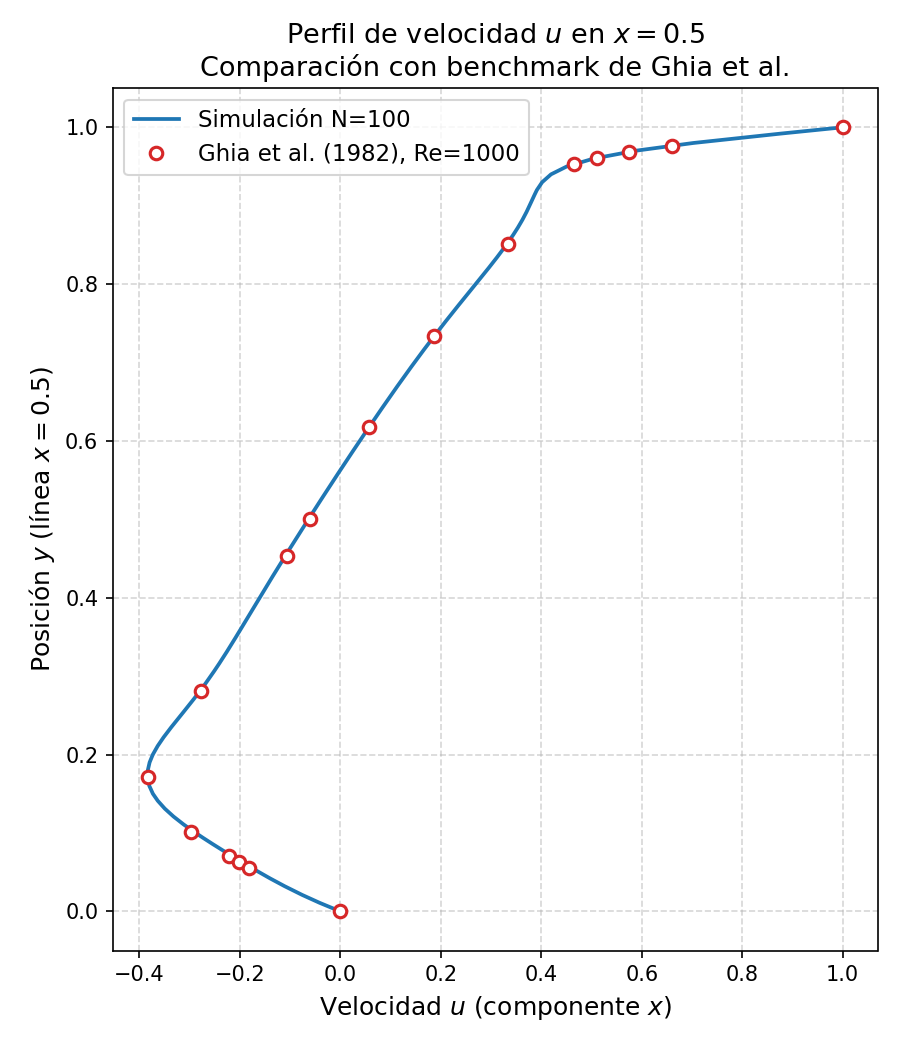
\includegraphics[width=0.5\textwidth]{ghia_comparison.png}

  \vspace{0.2cm}
  \textcolor{gray}{\small Re = 1000, malla 100$\times$100. Excelente concordancia con Ghia et al.}
\end{frame}

% ------------------------------------------------------------
\begin{frame}{Validación: DFG 2D-1 (Cilindro)}
  % Segundo benchmark: flujo alrededor de un cilindro en canal (Schäfer et al. 1996). Se validaron coeficientes de arrastre (CD) y sustentación (CL) contra valores de referencia. Error < 5%.

  \centering
  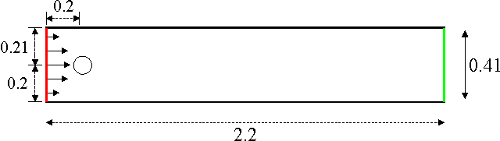
\includegraphics[width=0.45\textwidth]{dfg_geometry.png}

  \vspace{0.2cm}
  \textcolor{gray}{\small $Re = 20$, error en $C_D$, $C_L$ < 5\% respecto al benchmark}
\end{frame}

% ------------------------------------------------------------
\begin{frame}{Geometría: Estenosis parametrizable}
  % Se creó un generador de geometrías arteriales 2D con estenosis simétrica. Dos parámetros: severidad η (qué tan angosto) y pendiente α (qué tan abrupto). Las curvas de transición usan Bézier cúbicas. Mallado con GMSH (no estructurado y estructurado transfinito).

  \centering
  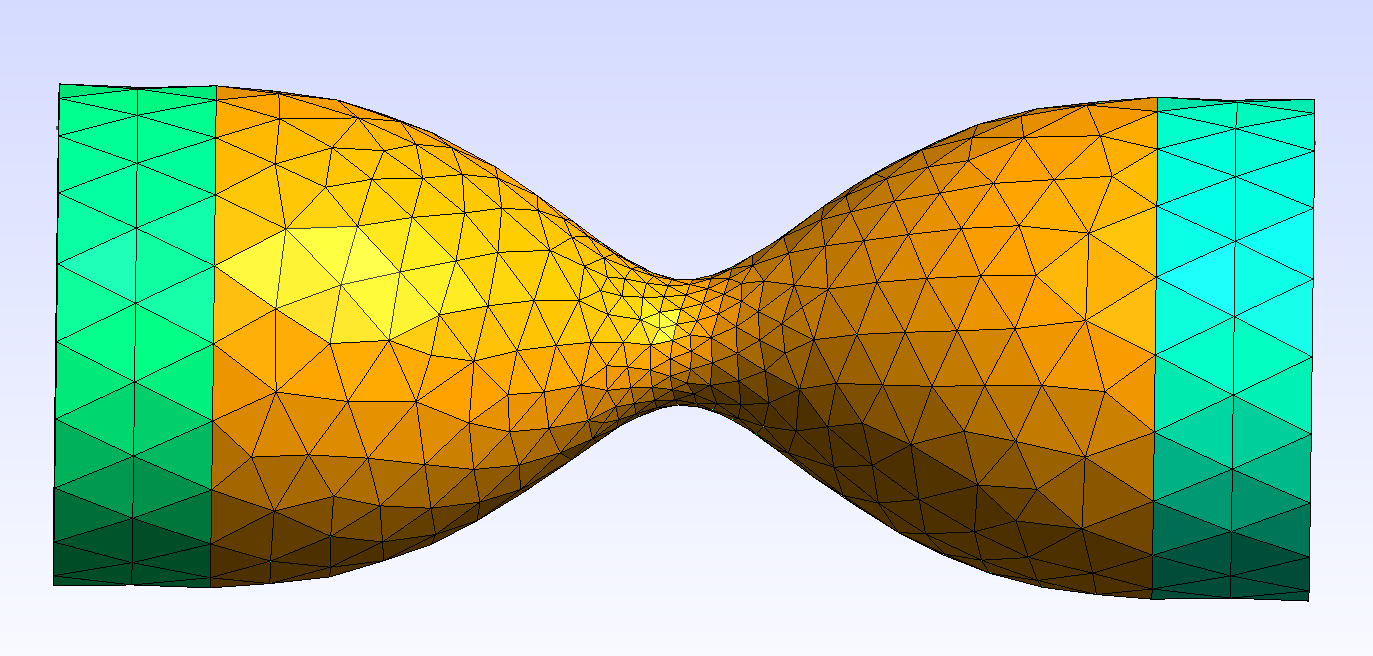
\includegraphics[width=0.9\textwidth]{geometria_arteria.png}

  \vspace{0.2cm}
  \textcolor{gray}{\small $\eta$: severidad de oclusión. $\alpha$: pendiente de transición.}
\end{frame}

% ------------------------------------------------------------
\begin{frame}{Geometría: Árbol microvascular}
  % Árbol simétrico generado con ley de Murray (r³ = 2·r_h³). Longitud proporcional al radio (L = λr). Ángulo de bifurcación de 35°. Tres niveles simulados explícitamente (hasta Re < 5). Resistencias distales modeladas analíticamente.

  \centering
  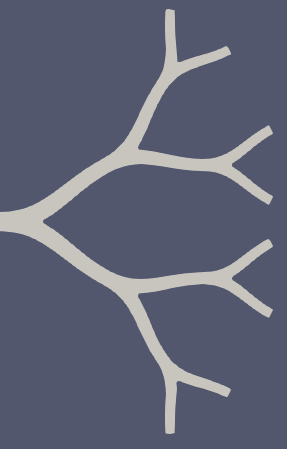
\includegraphics[width=0.45\textwidth]{geom_arbol.png}

  \vspace{0.2cm}
  \textcolor{gray}{\small Ley de Murray, 3 niveles explícitos, 27 generaciones totales}
\end{frame}

% ------------------------------------------------------------
\begin{frame}{Condiciones de frontera}
  % Inlet: presión débil (70 mmHg) + Nitsche para u_T = 0. Outlet: resistencia R (acoplamiento explícito Q^{n-1}). Backflow penalization para estabilidad. La resistencia del árbol no simulado se descuenta de la resistencia target.

  \centering
  \vfill
  \textbf{Inlet:} Presión $p_{in}=70$ mmHg + Nitsche ($u_T=0$)

  \vspace{0.2cm}
  \textbf{Outlet:} $p_{out} = R \cdot Q^{n-1}$

  \vspace{0.2cm}
  \textcolor{gray}{\small $R = R_{target} - R_{arbol}$}
  \vfill
\end{frame}

% ------------------------------------------------------------
\begin{frame}{Parámetros LAD}
  % Parámetros basados en la arteria descendente anterior izquierda (LAD). Longitud 138 mm, radios de entrada/salida fisiológicos. Presión diastólica 70 mmHg. Resistencia basal estimada ~13.79 g·s/mm.

  \centering
  \begin{tabular}{lc}
    \toprule
    Parámetro & Valor \\
    \midrule
    Longitud $L$ & 138 mm \\
    $R_{in}$ & 1.57 mm \\
    $R_{out}$ & 1.20 mm \\
    $p_{in}$ & 70 mmHg \\
    $\Delta t$ & $10^{-4}$ s \\
    $R_{base}$ & 13.79 g$\cdot$s/mm \\
    \bottomrule
  \end{tabular}
\end{frame}

% ------------------------------------------------------------
\section{Resultados}

% ------------------------------------------------------------
\begin{frame}{Estenosis baja vs alta severidad}
  % Severidad baja (η=0.25): flujo laminar, sin recirculación, estado estacionario rápido. Severidad alta (η=0.75): chorro de alta velocidad, inestabilidad transitoria, asimetría post-estenótica.

  \centering
  \includegraphics[width=0.8\textwidth]{flujo_severity_bajo_slope_bajo.pdf} \\
  \vspace{0.3cm}
  \includegraphics[width=0.8\textwidth]{flujo_severity_alto_estado_estacionario.pdf}

  \vspace{0.1cm}
  \textcolor{gray}{\small Arriba: $\eta=0.25$. Abajo: $\eta=0.75$.}
\end{frame}

% ------------------------------------------------------------
\begin{frame}{Artefacto de malla}
  % La asimetría post-estenótica con malla no estructurada resultó ser un artefacto numérico. Con malla estructurada transfinita que preserva simetría, el flujo permanece simétrico. FFR robusto (diferencia ~2%).

  \centering
  \includegraphics[width=0.9\textwidth]{figures/flujo_structured_severity75-tiff-converted-to.pdf}

  \vspace{0.2cm}
  \textcolor{gray}{\small Malla estructurada: flujo simétrico. FFR robusto ($\Delta < 2\%$).}
\end{frame}

% ------------------------------------------------------------
\begin{frame}{Esfuerzo cortante de pared (TAWSS)}
  % Zonas de bajo WSS (< 4 dyn/cm²) en región post-estenótica y bifurcaciones del árbol → condiciones pro-aterogénicas. Garganta de la estenosis: WSS elevado (> 15 dyn/cm²) → ateroprotector.

  \centering
  \includegraphics[width=0.9\textwidth]{presion_dist.pdf}

  \vspace{0.2cm}
  \textcolor{gray}{\small TAWSS $<$ 4 dyn/cm$^2$ en zonas post-estenóticas $\rightarrow$ pro-aterogénico}
\end{frame}

% ------------------------------------------------------------
\begin{frame}{Flujo y presión en el árbol microvascular}
  % Zonas de recirculación persistentes en la primera bifurcación. Distribución asimétrica del caudal en niveles profundos. Presión varía poco (43.4-44.0 mmHg) con incrementos localizados en bifurcaciones.

  \centering
  \includegraphics[width=0.45\textwidth]{flujo_arbol2.pdf}
  \hfill
  \includegraphics[width=0.45\textwidth]{presion_arbol.pdf}

  \vspace{0.2cm}
  \textcolor{gray}{\small Velocidad (izq.) y presión (der.) en el árbol microvascular}
\end{frame}

% ------------------------------------------------------------
\begin{frame}{Modelo de Ecuaciones Estructurales (SEM)}
  % Se derivó una variable latente: reducción de área relativa ΔA_rel = (2R²/L(R_in+R_out))·η²/α. Modelo SEM: FFR = -0.8885·ΔA_rel - 0.2004·η + 1.0238. R² = 0.8506. Ambas variables significativas (p < 0.05).

  \begin{table}
    \centering
    \small
    \begin{tabular}{lccc}
      \hline
      \textbf{Modelo} & $R^2$ & RMSE & MAE \\
      \hline
      \textbf{$\Delta A_{\text{rel}} + \eta$} & \textbf{0.8506} & \textbf{0.0283} & \textbf{0.0251} \\
      $\eta + \alpha$ & 0.7635 & 0.0356 & 0.0296 \\
      $\Delta A_{\text{rel}}$ & 0.6578 & 0.0428 & 0.0321 \\
      \hline
    \end{tabular}
  \end{table}

  \vspace{0.2cm}
  \textcolor{gray}{\small $\Delta A_{\text{rel}}$ captura la reducción de área integrada de la estenosis}
\end{frame}

% ------------------------------------------------------------
\begin{frame}{FFR predicho vs simulado}
  % Mostrar gráficamente la correlación entre FFR predicho por el SEM y FFR simulado. Los puntos se alinean bien con la identidad.

  \centering
  \vfill
  \textcolor{gray}{FFR$_{\text{pred}}$ = $-0.8885\Delta A_{\text{rel}} - 0.2004\eta + 1.0238$}

  \vspace{0.3cm}
  \textcolor{gray}{$R^2 = 0.85$ — buena capacidad predictiva \\ con costo computacional mínimo}

  \vfill
\end{frame}

% ------------------------------------------------------------
\begin{frame}{Impacto de la resistencia microvascular}
  % Experimento con 15 escenarios (muestreo estratificado por FFR, resistencias entre 13.79 y 20.19). Resultado: correlación Pearson r = -0.008 (p = 0.98). R² = 0.000068. La resistencia no explica el FFR.

  \centering
  \vfill
  \textbf{$r = -0.0082$} \quad $p = 0.9777$

  \vspace{0.2cm}
  \textbf{$R^2 = 0.000068$} \quad ($p = 0.2511$, prueba F)

  \vspace{0.5cm}
  \textcolor{gray}{\small La resistencia microvascular NO se correlaciona con el FFR \\ en el rango evaluado}
  \vfill
\end{frame}

% ------------------------------------------------------------
%\begin{frame}{FFR vs Resistencia microvascular}
%  % Gráfico de dispersión FFR vs R. No se observa tendencia. Los puntos se distribuyen horizontalmente. La línea de regresión es casi plana.
%
%  \centering
%  \textcolor{gray}{FFR vs Resistencia: sin correlación aparente}
%\end{frame}

% ------------------------------------------------------------
\section{Discusión}

% ------------------------------------------------------------
\begin{frame}{Interpretación fisiológica}
  % Bajo hiperemia máxima, la resistencia microvascular se minimiza y estabiliza. El FFR refleja exclusivamente la severidad de la estenosis epicárdica. Nuestros resultados confirman esta premisa: el FFR está dominado por la geometría.

  \centering
  \vfill
  {\large\textbf{FFR dominado por la geometría de la estenosis}}

  \vspace{0.5cm}
  \textcolor{gray}{\small La impedancia hidráulica de la lesión es el factor determinante \\ del gradiente de presión bajo hiperemia máxima}

  \vfill
\end{frame}

% ------------------------------------------------------------
\begin{frame}{Limitaciones del modelo}
  % Paredes rígidas (sin FSI) → sobreestima caída de presión 27-37% (Konala). Newtoniano → subestima caída 8-12% (Dutra). 2D vs 3D. Condiciones de frontera fijas. Sin tono vasomotor dinámico.

  \centering
  \vfill
  \textcolor{gray}{Paredes rígidas (sin FSI)} \\
  \textcolor{gray}{Fluido newtoniano} \\
  \textcolor{gray}{Dominio 2D} \\
  \textcolor{gray}{Sin acoplamiento fluido-estructura}

  \vspace{0.3cm}
  \textcolor{gray}{\small Limitaciones que pueden ocultar efectos microvasculares}
  \vfill
\end{frame}

% ------------------------------------------------------------
\section{Conclusiones}

% ------------------------------------------------------------
\begin{frame}{Conclusiones (1)}
  \begin{itemize}
    \item {\color{gray} Plataforma de simulaci\'on hemodin\'amica parametrizable implementada y validada}
    \item {\color{gray} Modelo SEM predice FFR con $R^2 = 0.85$ a partir de la morfología de la estenosis}
    \item {\color{gray} La resistencia microvascular no mostró correlación significativa con el FFR bajo hiperemia máxima}
  \end{itemize}
\end{frame}

% ------------------------------------------------------------
\begin{frame}{Conclusiones (2)}
  \begin{itemize}
    \item {\color{gray} Zonas de bajo WSS ($<$ 4 dyn/cm$^2$) identificadas en regiones post-estenóticas y bifurcaciones → pro-aterogénicas}
    \item {\color{gray} La representaci\'on expl\'icita de la microvasculatura no altera significativamente la predicci\'on del FFR}
    \item {\color{gray} El enfoque param\'etrico es computacionalmente eficiente e interpretable f\'isicamente}
  \end{itemize}
\end{frame}

% ------------------------------------------------------------
\begin{frame}[plain]
  \centering
  \vfill
  {\Large\textbf{Gracias}}

  \vspace{0.5cm}
  \textcolor{gray}{Código: \href{https://github.com/JuanJoZP/cfd-hemodynamic}{github.com/JuanJoZP/cfd-hemodynamic}}

  \vfill
\end{frame}

\end{document}
